\chapter{Solution} To build an effective and easy to use hand gesture recognition system for NAO, various tools and technologies were studied during this thesis. Figure \ref{fg:hri:components} shows the individual components which are essential parts of this thesis in implementing the goal. The main challenge is to find a solution that can integrate all these components into a robust system. However, due to the computational and compatibility limitations of NAO, we have faced problems in implementing few contemplated solutions which are described in the next section. Finally, the successful solution in achieving the goal will be discussed in the following sections.

\begin{figure}
	[h] \centering 
	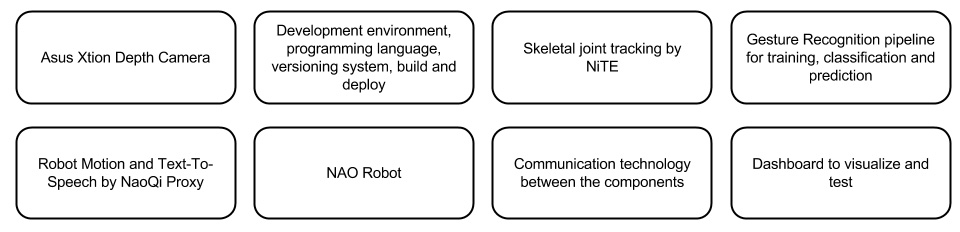
\includegraphics[height=35mm]{figures/content/hri-components.jpg} \caption{Component} \label{fg:hri:components} 
\end{figure}


\section{Experimental Designs} 
\subsection{Everything On-Board} First experiment design was conceived in a way that depth camera, skeletal joint tracking, gesture recognition infrastructure and robot motion will be embedded into the on-board computer of NAO. However, gesture recognition infrastructure is composed of computationally intensive machine learning processes and along with skeletal joint tracking by NiTE had pushed NAO to 100 $ \% $ CPU load consistently. --- Show htop of NiTE cpu consumption ----

\subsection{Extending NAO with Single Board Computer} In order to escape the computational limitation of NAO, another experimental design was contemplated, that the robot will be extended as shown in the figure \ref{fg:nao:bag} with a powerful Single Board Computer such as pcDuino or RaspberryPi. However, Asus Xtions higher power consumption of 2.5 Watts with weight of 250 grams, pcDuinos power consumption of 2A at 5VDC with weight of 100 grams and additional weight by 3D printed mounts, heat sinks and wires will make NAO to be heavier and ultimately result in poor motion performances and higher power consumption. 

\begin{figure}
	[h] \centering 
	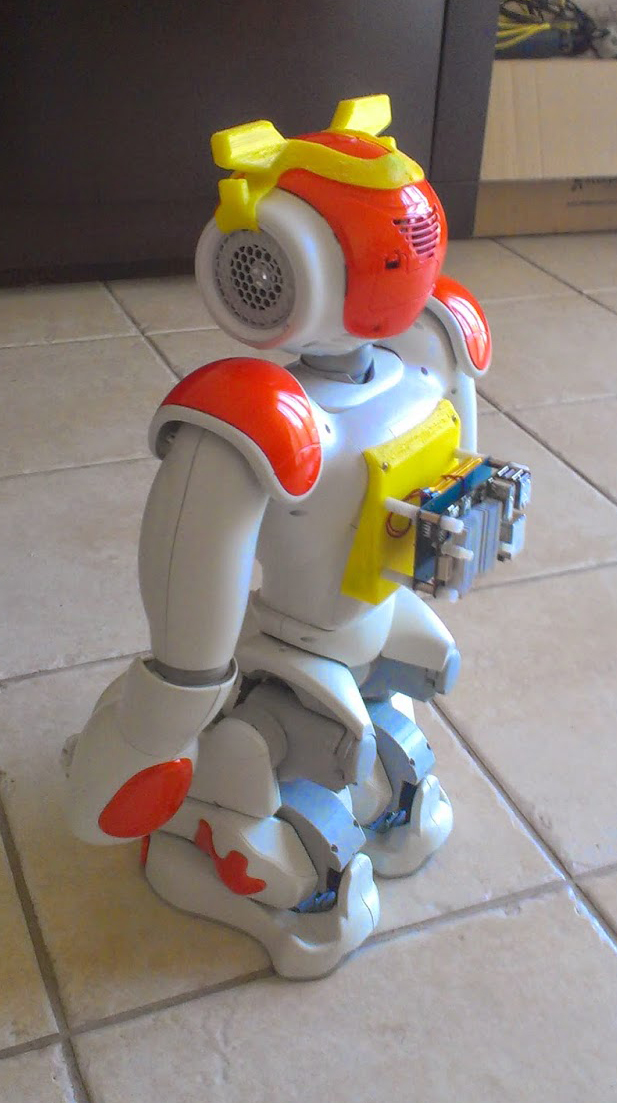
\includegraphics[height=7cm]{figures/content/nao-bag.jpg} \caption{3D printed mount to extend NAO with an external Single Board Computer. \cite{19} } \label{fg:nao:bag} 
\end{figure}


\subsection{Everything Off-Board} This experimental design pushes all the components to an off-board computer that could be a PC connected with depth camera at a fixed location. User will gesticulate in front of the camera and all processing will be done on PC. Finally predicted gesture will be transformed into a motion and voice, and it will be sent to NAO via Aldebaran proxies using WLAN. This design completely decouples the robot from other components and degrades the natural interaction between human and the robot. However, this design will suit for other applications such as indoor navigation and localization of NAO.

\section{Implementation } After analyzing the disadvantages of other experimental designs, the final design was chosen to build an efficient real-time hand gesture recognition for human-robot interaction using skeletal points. Figure \ref{fg:hri:architecture} shows the architecture of the solution that was implemented during this thesis by grouping many components into 4 different modules which serve various purposes. Each module is implemented in different environment as shown in the figure and they communicate with one another to complete the data flow. All these modules uses a common configuration file that contains information such as port number, host name and log path.

\begin{figure}
	[h] \centering 
	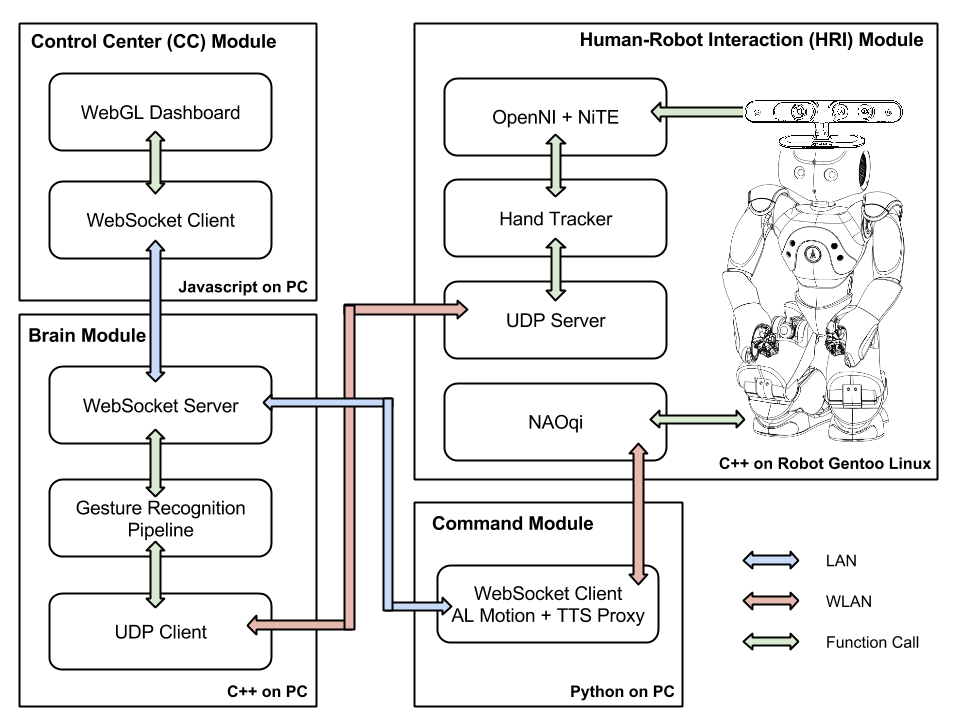
\includegraphics[height=11cm]{figures/content/hri-architecture.png} \caption{HRI Architecture} \label{fg:hri:architecture} 
\end{figure}


\subsection{Human-Robot Interaction (HRI) Module} HRI module is implemented first in order to get the raw data from the depth sensor and process it to track the skeletal joint positions in real world coordinates. It developed in C++ using a core library called Boost and NiTE 2 framework is used for the purpose of skeletal joints tracking. This module is deployed on the general purpose computer that is running inside the robot with necessary libraries and drivers.

Boost is a set of libraries for the C++ programming language that provide support for tasks and structures such as linear algebra, pseudo random number generation, multi threading, image processing, regular expressions, and unit testing. It contains over eighty individual libraries.

HRI module is composed of 3 components which are UDP Server, Gesture and Skeleton tracker. Flowchart \ref{fg:hri:flow} shows the data flow of this module where the user is asked to select Gesture or Skeleton tracker, when the program is started. It creates 2 threads depending on the selection: 

\begin{itemize}
	\item UDP Server thread - Asynchronously send data to the client and thread is always running.
	\item Gesture or Skeleton tracker thread - A loop in the thread polls for a new frame from the depth camera till some key is pressed. If loop is interrupted, then the thread is exited and finally program is closed.

\end{itemize}

Gesture and Skeleton tracker serve the purpose in extracting features from the raw data to implement a hand gesture recognition system. However, Skeleton tracker tracks 15 skeletal points in the human body and that leads to very intensive computation. Due to processing limitations of NAO, we chose to use Gesture tracker as it tracks only hand joints. Following sections describe internal working HRI module.

\begin{figure}
	[h] \centering 
	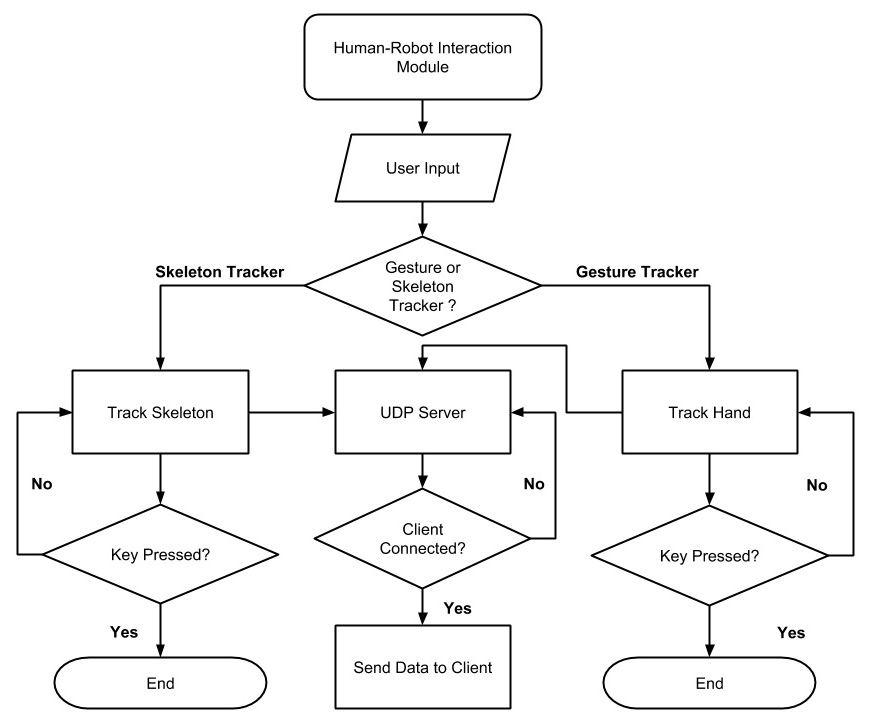
\includegraphics[height=115mm]{figures/content/hri-flow.jpg} \caption{HRI Module Control Flow} \label{fg:hri:flow} 
\end{figure}


\subsubsection{UDP Server}
HRI module has to process the raw information from the depth camera and it has to send it to Brain module for the purpose of gesture recognition. As show in the architecture diagram \ref{fg:hri:architecture}, Brain module must be connected via Wireless Local Area Network (WLAN). WLAN at 2.4GHz readily is available on NAO and lead us to a solution, where we have to choose an UDP protocol to transmit the processed data from depth camera. UDP was chosen over other protocols because depth camera produces 30 depth images per second and transferring such a large amount of data using conventional communication technologies such as TCP will be create much overhead and delay in the communication.

Due to asynchronous requirement of the server, Boost Asio library is used to implement UDP server. Boost.Asio is a cross-platform C++ library for network and low-level I/O programming that provides developers with a consistent asynchronous model using a modern C++ approach.

UDP Server is basically an asynchronous programs that creates an UDP socket and listens to an port on the local machine. In this case, we have created a common configuration file that contains port numbers for each module in this project. Therefore, this server listens to the 5005 on NAO and waiting for the clients to connect. 

Once the client is connected, it stores the endpoint details of the client such as IP address and the port number of the UDP client (Brain module), so that it can communicate with the Brain module whenever there is some data to be transmitted. Asynchronous functionality Boost.Asio calls the callback handler only when there is communication with the clients and waits in the thread for the next communication.

\subsubsection{Gesture Tracker} \label{sec:hri:ges}
Gesture tracker is a component of HRI module that makes use of NiTE framework to localize the hand of user in the field of view and track the hand position till the hand leaves the field of view (FOV) or hand is touching another object or hidden by an object. 

It uses HandTracker class of NiTE framework and it needs to go through following steps before it can track a hand. Section \ref{sec:nite} discusses extensively about the functionalities of NiTE framework.

\begin{itemize}
	\item NiTE framework must be initialized using nite::initialize() function.
	\item Depth camera must be connected and nite::HandTracker must be created using OpenNI compatible  device id. If not, default depth camera will be selected.
	\item NiTE Focus Gestures such as Wave or Click detection must be initiated in order to localize the hand at first.
	\item nite::HandTrackerFrameRef must be read continuously for a new gesture.
	\item If Wave or Click gesture is detected, then hand tracking will be started using the position of hand that triggered the gesture.
\end{itemize}

Once the hand is been tracked, the hand will be added an id and it will be added to HandTrackerFrameRef. NiTE framework allow users to add many number of hands and it will be tracked till there is enough computation power and hands are not overlapping. HandTrackerFrameRef contains the array of all active hands and every hand is an object of nite::HandData. It contains the position of the hand in 3 dimensional float stored in a class called Point3f.

Unlike nite::UserTracker, HandTracker class can return only the hand position in the space and it can not specify whether it is a left or right hand. It is very necessary information for hand gesture training and classification because confused hand names will lead to a false model of the hand gesture and ultimately resulting in a bad performance. Hence, we have implemented a simple logic with the help of an assumption that user will gesticulate the focus gesture (Wave or Click) only in the order of right hand first and left hand second. 

Four integer variables leftHand, rightHand, lastLostHand and handsSize are used to find whether tracked or hand is left or right. The logic behind is that when handsSize and lastLostHand is zero and a new hand is found, that is considered as right hand and its nite::HandData::HandId is stored in the variable rightHand. Respectively, the next hand is stored as leftHand and handsSize counter is increased. If a hand is lost or not tracking, then lastLostHand will be updated with the id of the hand that was lost. When there is a new hand and handsSize and lastLostHand are not zero, then new handId will be set to leftHand or rightHand based on lastLostHand variable.

However, functionalities gesture tracker are not only  to track hand, but also send these information to Brain module via UDP. Therefore, C++  nite::HandData objects must be serialized before transmitted over the network. Therefore, we chose JSON serialization and send them across the network as strings as shown in \ref{code:hand:data}

\begin{lstlisting}
	{
		"RIGHT": ["275.456", "339.026", "1841.850"], 
		"LEFT": ["-456.289", "353.880", "1761.360"]
	}
\end{lstlisting}
\label{code:hand:data}

Furthermore, HRI module send informations such as detected focus gesture and info messages to Brain module as shown in \ref{code:hand:info} to be displayed on the control center dashboard. Info messages helps us to know the status of computationally intensive hand tracking algorithm which is the core component of HRI module. 

\begin{lstlisting}
{"GESTURE":"WAVE"}
{"GESTURE":"CLICK"}
{"INFO": "Found new hand with id 1"}
{"INFO": "LEFT Hand is lost"}
{"INFO": "RIGHT Hand is lost"}
{"INFO": "Both hands are lost"}
{"INFO": "LEFT Hand is at FOV"}
\end{lstlisting}
\label{code:hand:info}

\subsubsection{Skeleton Tracker}
Skeleton Tracker is a component of HRI module that is more complex and computational intensive, since it uses nite::UserTracker to track 15 bone joints of human body. Like Gesture Tracker in the section \ref{sec:hri:ges}, this component has to follow few procedure before tracking and it starts with an UDP server to unicast joint positions to Brain module.
 
 \begin{itemize}
 	\item NiTE framework must be initialized using nite::initialize() function.
 	\item Depth camera must be connected and nite::UserTracker must be created using OpenNI compatible  device id. If not, default depth camera will be selected.
 	\item Pose in front the camera as shown in the figure \ref{fg:ni:skeleton} to let the algorithm calibrate the body position. 
 	\item nite::UserTrackerFrameRef must be read continuously for a new user and if a new user is found, skeleton tracking will be started.
 \end{itemize}
 
 \begin{figure}
	[h] \centering 
	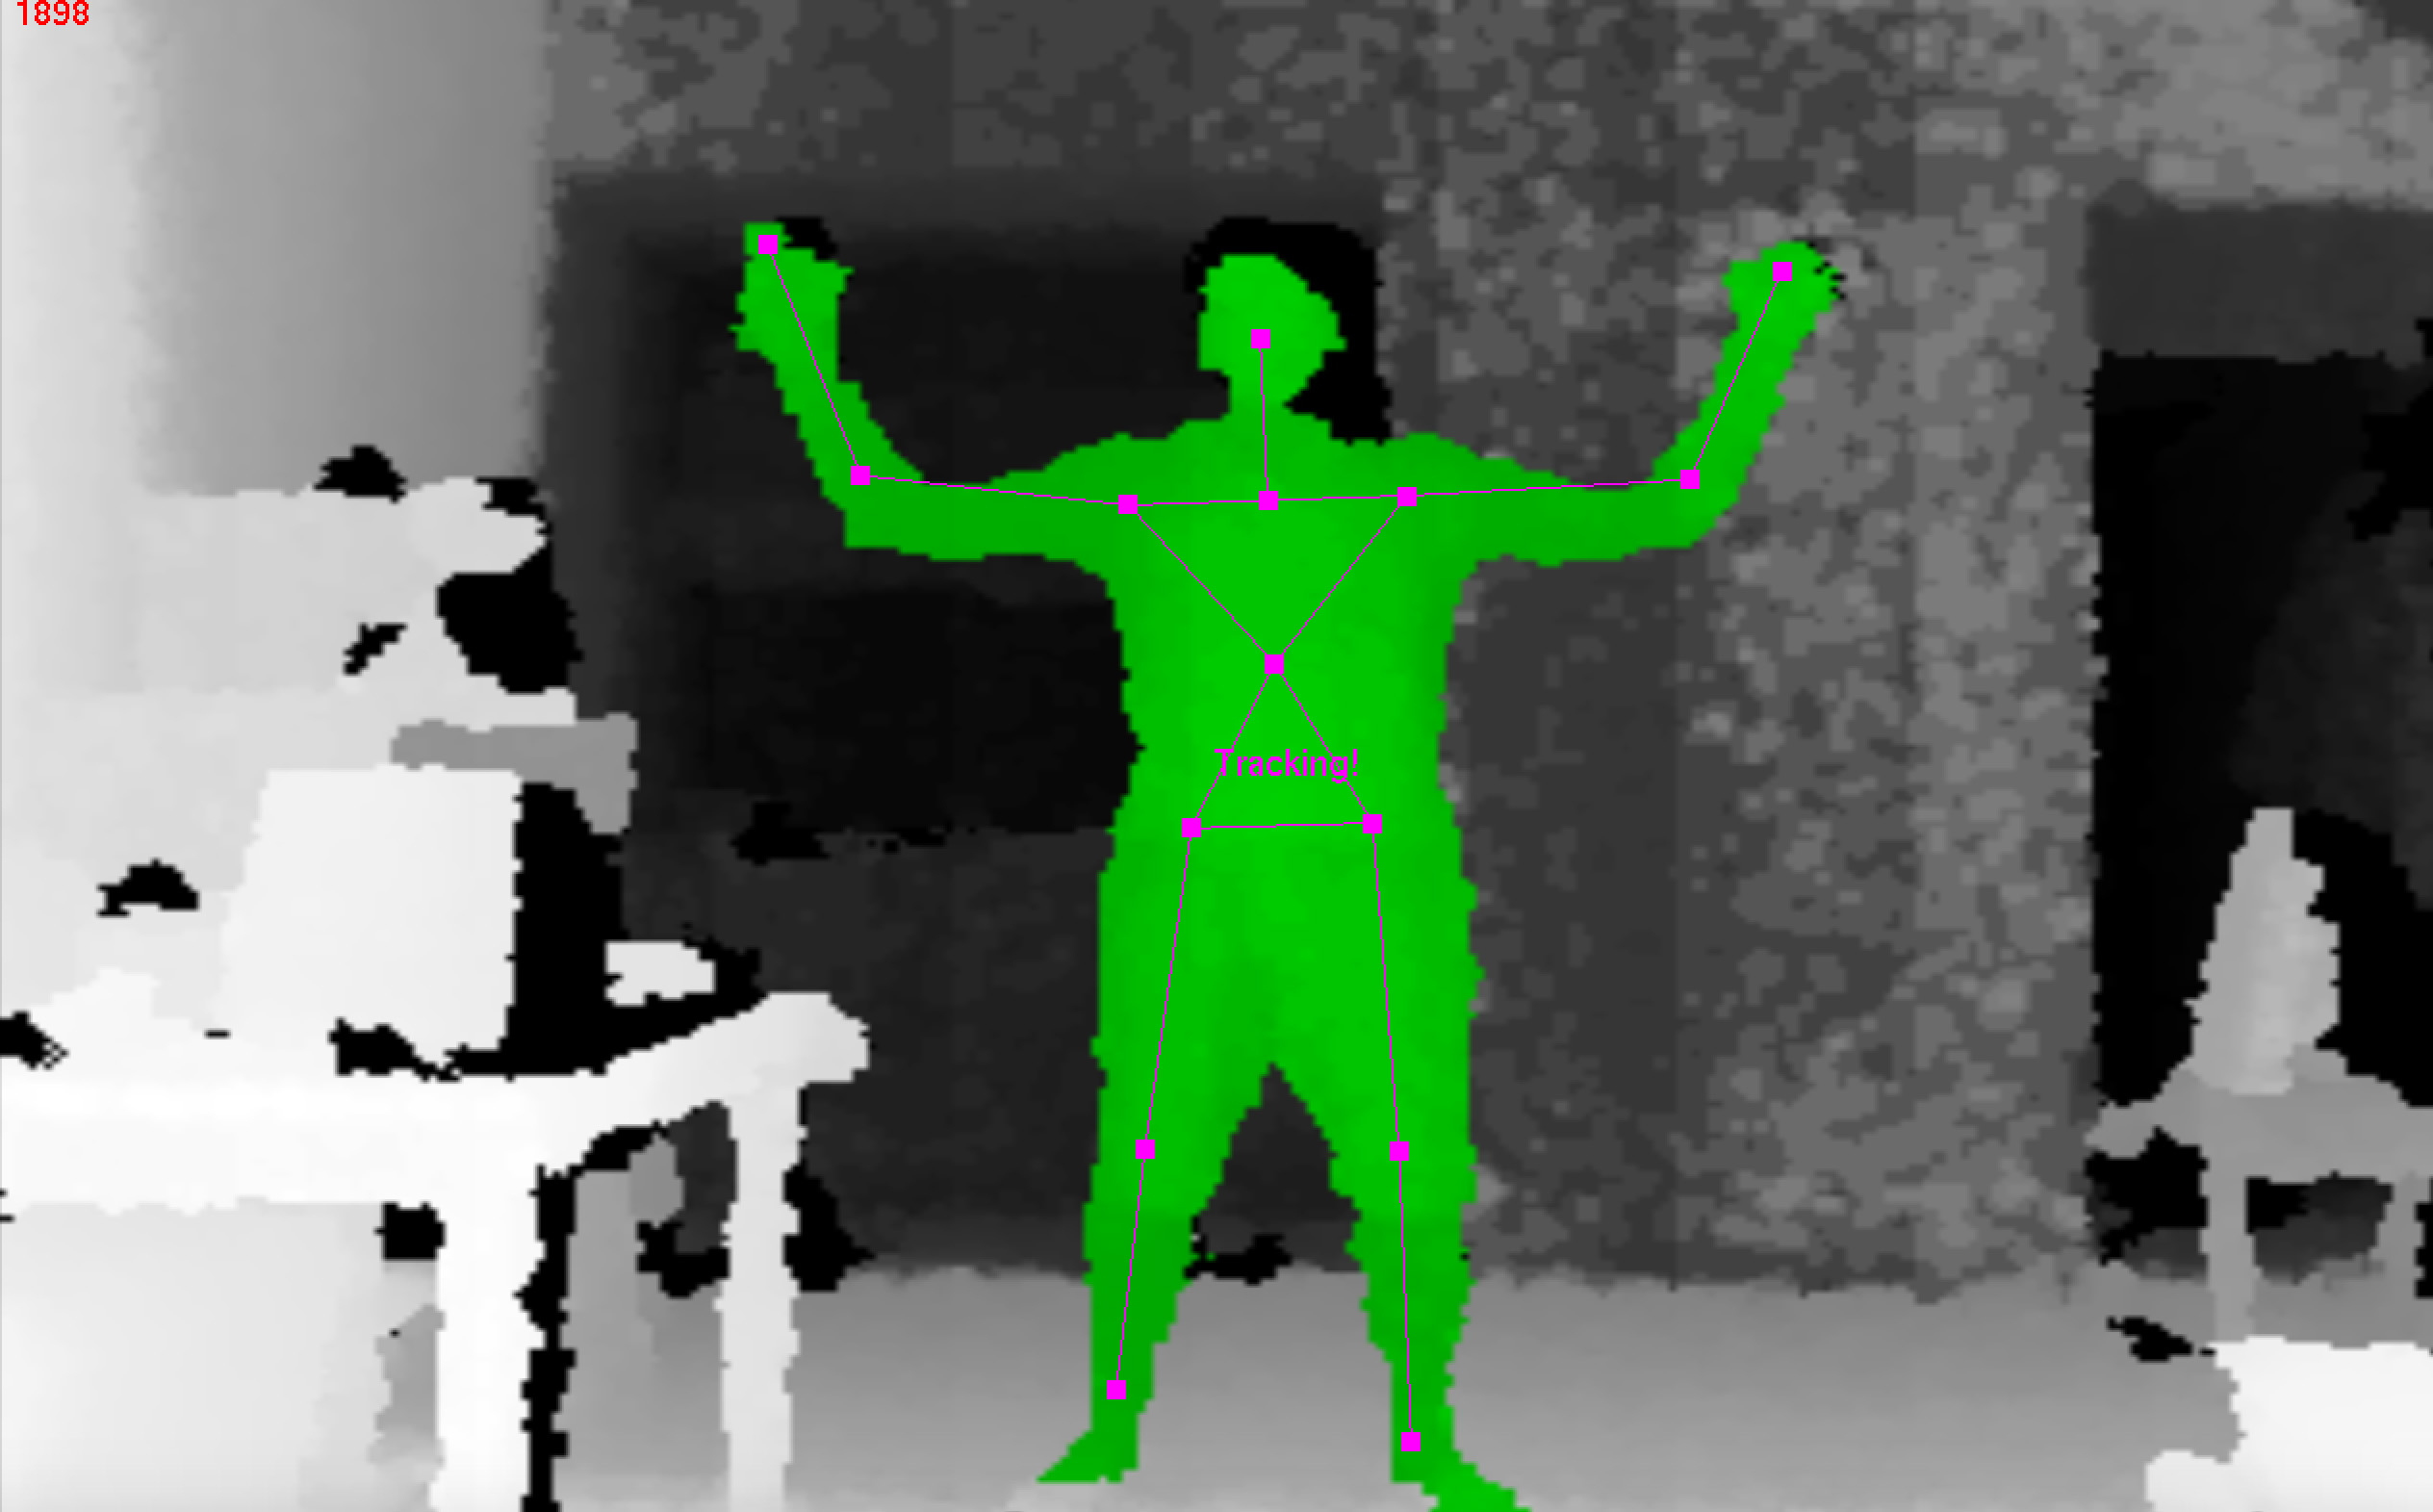
\includegraphics[width=145mm]{figures/content/ni-skeleton.jpg} \caption{Image captured while NiTE tracks 15 skeletal joints of the user using depth camera Asus Xtion. } \label{fg:ni:skeleton} 
\end{figure}

 
 Unlike nite::HandTracker, UserTracker class of NiTE uses complex algorithms to keep tracking the skeleton even when the user poses in many ways. Therefore, it needs the data provided by NiTE framework which contain 1 million training samples. In addition, UserTracker can return 15 skeletal joints position and orientation and they are labeled by the joint name. This feature helps us to avoid the implementation to find the hand name. Moreover, details of joint orientations offer us a chance to calculate positions not only in Cartesian coordinates, but also in spherical coordinates system which is essential for many complex hand gesture recognition solutions. Furthermore, SkeletonJoint class indicates how sure the NiTE skeleton algorithm is about the position data stored about the joint. The value is between 0 and 1, with increasing value indicating increasing confidence. Section \ref{sec:nite} discusses extensively about the algorithm of NiTE.
 
 Finally, Skeleton tracker serializes the C++ nite::UserData objects to JSON in strings  as shown in \ref{code:skeleton:data} in order to asynchronously transfer to the client for further gesture recognition procedures.
 
 \begin{lstlisting}
	{
		"HEAD": ["-274.5578", "583.2249", "1933.924"],
		"NECK": ["-286.0945", "471.8282", "1996.656"],
		"LEFT_SHOULDER": ["-399.2939", "453.2498", "1975.477"],
		"RIGHT_SHOULDER": ["-172.895", "490.4066", "2017.835"],
		"LEFT_ELBOW": ["-673.5372", "389.9277", "1973.389"],
		"RIGHT_ELBOW": ["77.3149", "437.1607", "2201.007"],
		"LEFT_HAND": ["-950.7228", "362.1895", "1930.967"],
		"RIGHT_HAND": ["351.137", "509.7826", "2453.827"],
		"TORSO": ["-258.3584", "272.1229", "2023.593"],
		"LEFT_HIP": ["-321.3845", "57.52153", "2033.549"],
		"RIGHT_HIP": ["-139.8603", "87.31343", "2067.511"],
		"LEFT_KNEE": ["-313.5818", "-344.5291", "2039.209"],
		"RIGHT_KNEE": ["-129.7786", "-280.5863", "2110.95"],
		"LEFT_FOOT": ["-341.4384", "-665.9058", "2189.055"],
		"RIGHT_FOOT": ["-172.1151", "-559.3973", "2262.547"]
	}
 \end{lstlisting}
 \label{code:skeleton:data}
 
\subsection{Brain Module} Brain module is the core functional part of this thesis. It is named as Brain since it refers to the anatomical brain that plays the vital role of the human life in learning, classifying, predicting and decision making. 

\begin{figure}
	[h] \centering 
	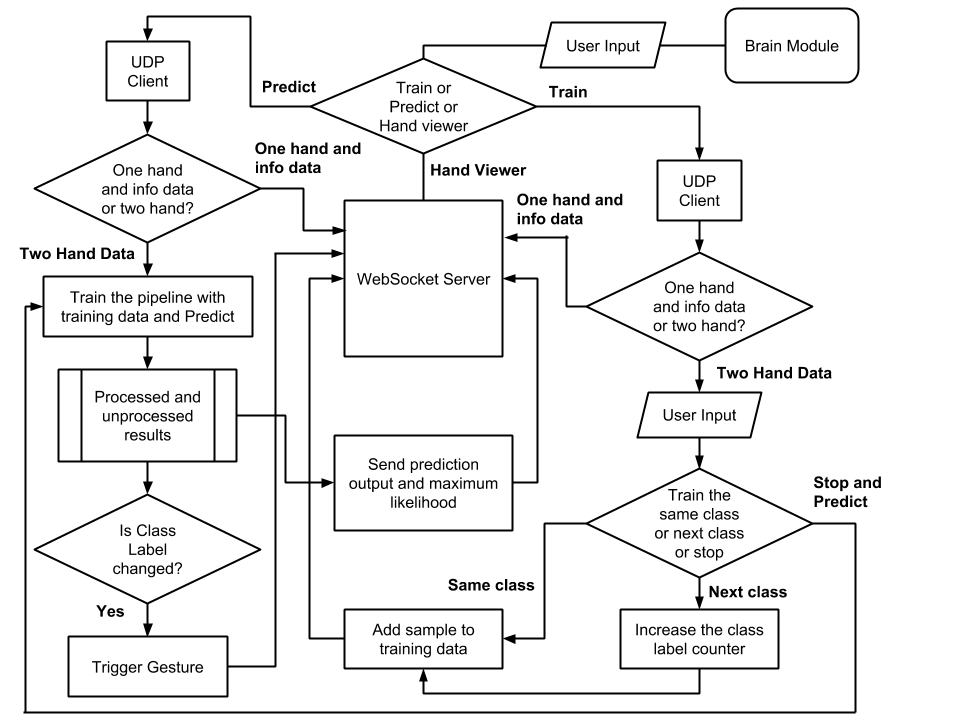
\includegraphics[height=115mm]{figures/content/brain-flow.png} \caption{Brain Module Control Flow} \label{fg:brain:flow} 
\end{figure}


\subsection{Control Center (CC) Module}

\subsection{Command Module} 
